\section{Dataset}
\label{sec:dataset}
% \todo[inline]{Dominik}

% weniger bilder am rand von kleinen objekten, aufgrund des bildänderungsalgorithmuses (siehe kapitel ...)
% all the different objects
% some pictures to illustrate something
% stats (from python file)

% ref to picture of lamp brightness distribution (camera / lighting)



\begin{table}[h]
  \caption{List of the different objects}
  \label{tab:objects}
  \centering
  \begin{tabular}{lll}
    \toprule
    \textbf{Objects} &  &  \\
    \midrule
	Nerf Dart & Spiky Ball & Stuffed Bunny \\
	American Football & Tesafilm & Goalkeeper Glove \\
	Table Tennis Ball & Sponge & Hemp Cord \\
	Shuttlecock & Lego Duplo Brick (Red) & Paper Ball \\
	Sporf & Lego Duplo Brick (Green) & Beer Cap \\
	Arrow & Lego Duplo Figure & Water Bottle \\
	Hand Featherball & Foam Dice &  \\
	Floorball & Infant Shoe &  \\
    \bottomrule
  \end{tabular}
\end{table}


\begin{figure}[ht]
  \centering
  \begin{subfigure}[b]{0.45\textwidth}
    \centering
    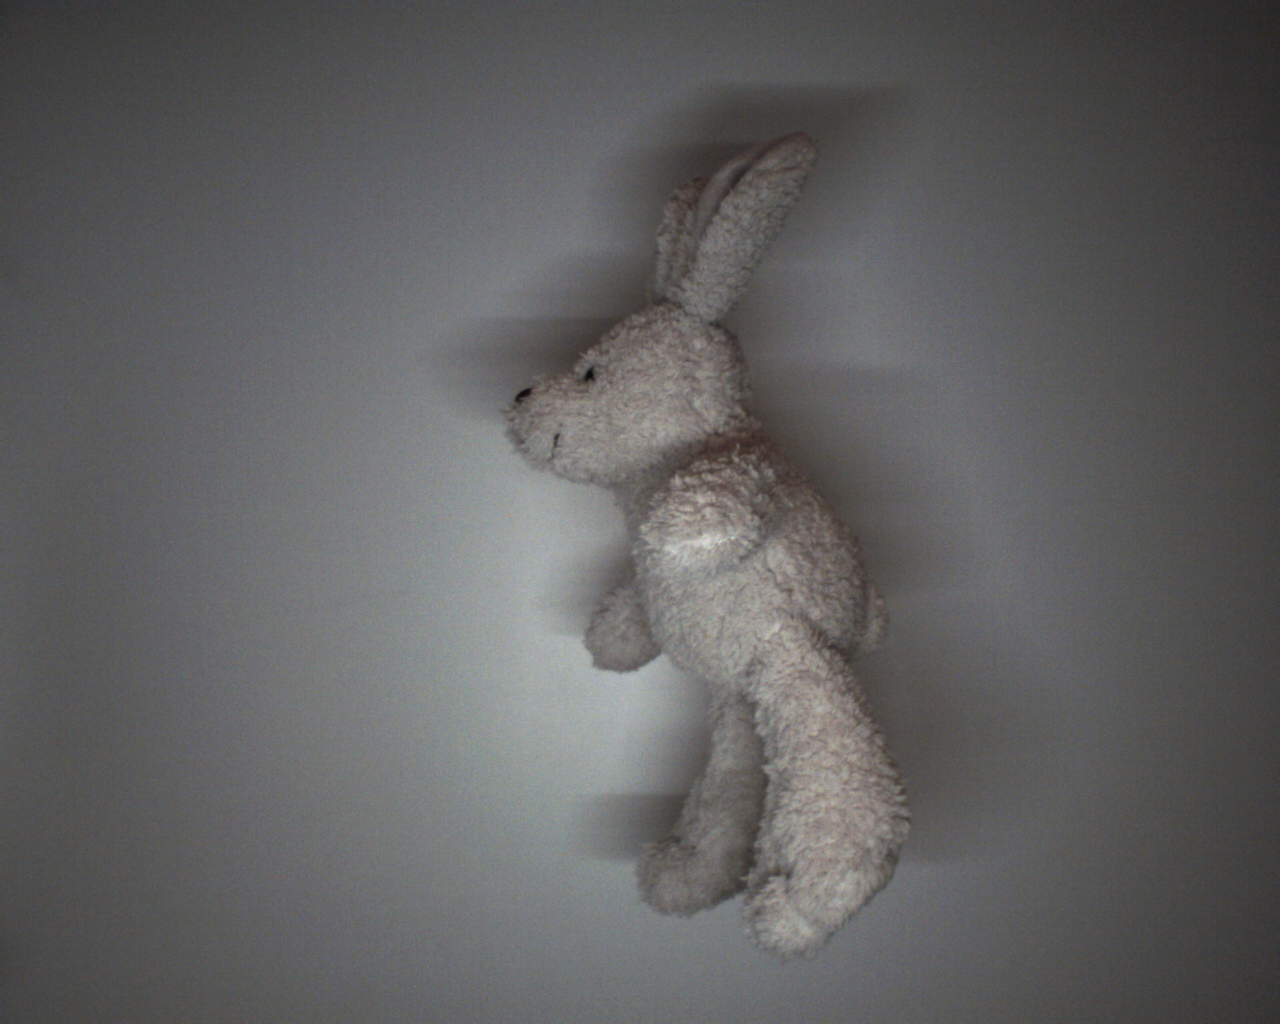
\includegraphics[width=0.9\textwidth]{1574952009_278_10_stuffed-bunny}
    \caption{Stuffed Bunny}
    \label{subfig:stuffed_bunny}
  \end{subfigure}
  \begin{subfigure}[b]{0.45\textwidth}
    \centering
    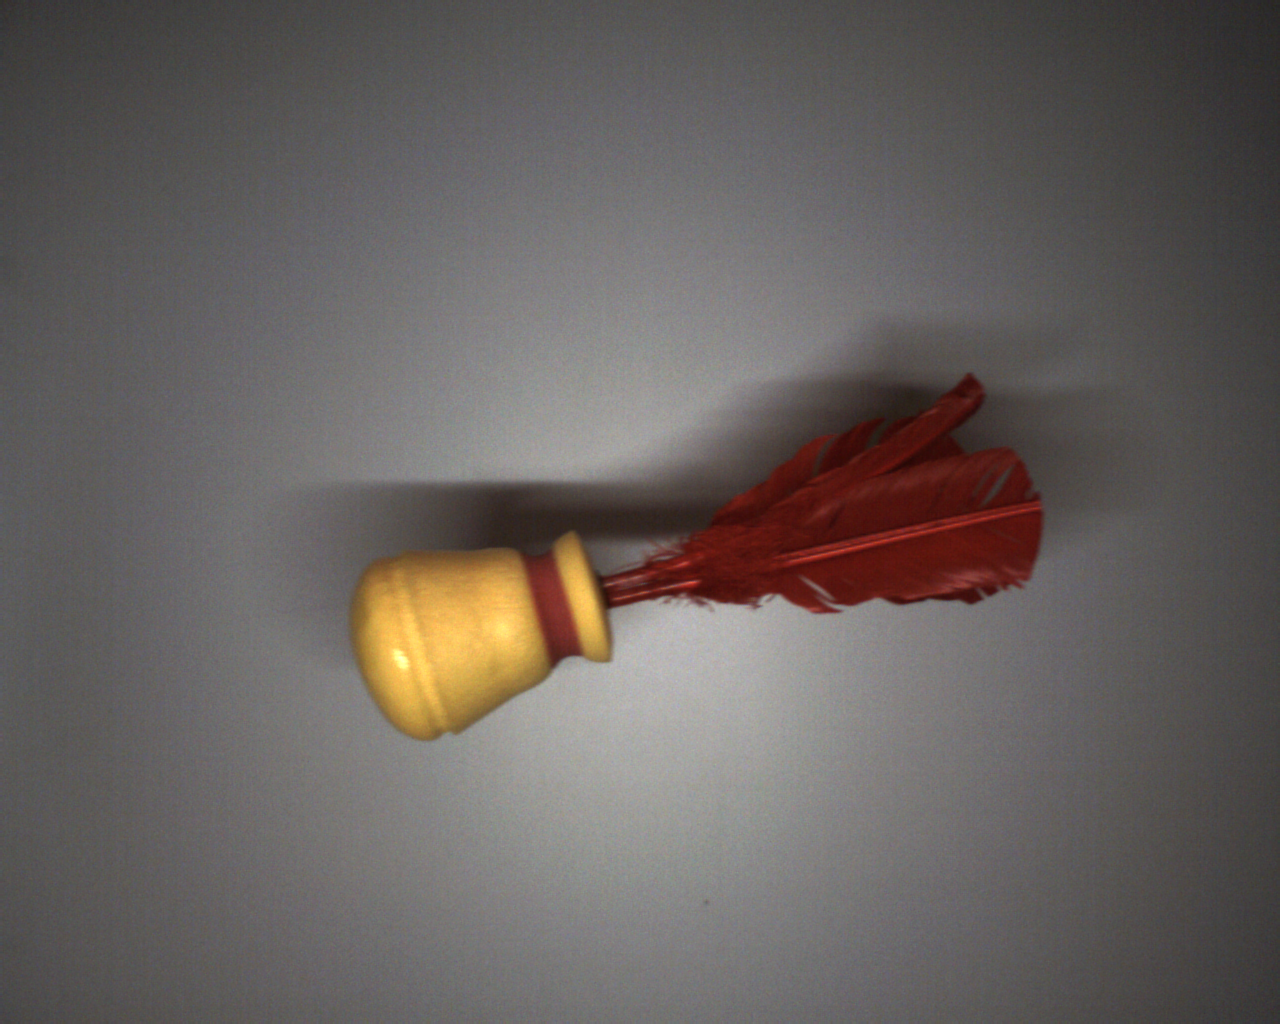
\includegraphics[width=0.9\textwidth]{1574943825_125_8_hand-featherball}
    \caption{Hand Featherball}
    \label{subfig:hand_featherball}
  \end{subfigure}
  \caption{Two pictures from the dataset}
  \label{fig:dataset}
\end{figure}

% Two-Row table
% Nerf Dart & Lego Duplo Brick (Red) \\
% American Football & Lego Duplo Brick (Green) \\
% Table Tennis Ball & Lego Duplo Figure \\
% Shuttlecock & Foam Dice \\
% Sporf & Infant Shoe \\
% Arrow & Stuffed Bunny \\
% Hand Featherball & Goalkeeper Glove \\
% Floorball & Hemp Cord \\
% Spiky Ball & Paper Ball \\
% Tesafilm & Beer Cap \\
% Sponge & Water Bottle \\
